\noindent
\begin{minipage}[t]{0.25\textwidth}
    \vspace{0pt}%
    \vspace{74pt}%
    {\small
    \noindent Hình 14 biểu diễn đồ thị của hàm số $f$ trong Ví dụ 7(b). Đồ thị này củng cố cho kết quả của chúng ta vì có một tiếp tuyến ngang khi $x = 1{,}5$ [tại đó $f'(x) = 0$] và một tiếp tuyến đứng khi $x = 0$ [tại đó $f'(x)$ không xác định].\par
    }

    \vspace{12pt}
    \noindent
    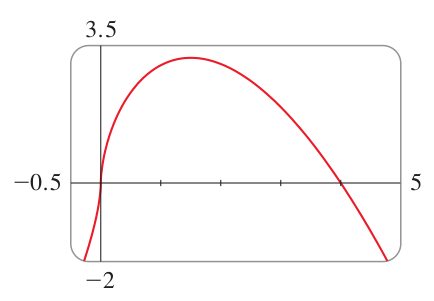
\includegraphics[width=\linewidth]{images/p0319_fig1.png}

    \vspace{3pt}
    \noindent\textbf{\textsf{HÌNH 14}}
\end{minipage}%
\hfill
\begin{minipage}[t]{0.71\textwidth}
    \vspace{0pt}%
    \begin{definitionbox}
    \noindent\stewartboxnum{6}\quad\textbf{\color{stewartred}Định nghĩa}\quad Một \textbf{số tới hạn} của hàm số $f$ là một số $c$ thuộc tập xác định của $f$ sao cho $f'(c) = 0$ hoặc $f'(c)$ không tồn tại.
    \end{definitionbox}

    \vspace{9pt}
    \noindent\textbf{\textsf{\color{stewartcyan}VÍ DỤ 7}}\quad Tìm các số tới hạn của (a) $f(x) = x^3 - 3x^2 + 1$ và (b) $f(x) = x^{3/5}(4 - x)$.

    \vspace{5pt}
    \noindent\textbf{\textsf{\color{stewartcyan}LỜI GIẢI}}\quad\textbf{(a)}~Đạo hàm của $f$ là $f'(x) = 3x^2 - 6x = 3x(x - 2)$. Vì $f'(x)$ tồn tại với mọi $x$, các số tới hạn duy nhất của $f$ xuất hiện khi $f'(x) = 0$, nghĩa là khi $x = 0$ hoặc $x = 2$.

    \vspace{4pt}
    \noindent\textbf{(b)}~Trước tiên lưu ý rằng tập xác định của $f$ là $\mathbb{R}$. Quy tắc nhân cho ta
    \begin{align*}
    f'(x) &= x^{3/5}(-1) + (4 - x)\left(\tfrac{3}{5}x^{-2/5}\right) = -x^{3/5} + \frac{3(4 - x)}{5x^{2/5}} \\[4pt]
    &= \frac{-5x + 3(4 - x)}{5x^{2/5}} = \frac{12 - 8x}{5x^{2/5}}
    \end{align*}
    [Cùng kết quả này có thể thu được bằng cách trước hết viết $f(x) = 4x^{3/5} - x^{8/5}$.] Do đó $f'(x) = 0$ nếu $12 - 8x = 0$, tức là $x = \frac{3}{2}$, và $f'(x)$ không tồn tại khi $x = 0$. Vậy các số tới hạn là $\frac{3}{2}$ và $0$.\hfill{\color{stewartcyan}$\blacksquare$}

    \vspace{7pt}
    \noindent Dưới góc độ các số tới hạn, Định lý Fermat có thể được phát biểu lại như sau (so sánh Định nghĩa 6 với Định lý 4):

    \vspace{5pt}
    \begin{definitionbox}
    \noindent\stewartboxnum{7}\quad\textit{Nếu $f$ đạt cực đại địa phương hoặc cực tiểu địa phương tại $c$, thì $c$ là một số tới hạn của $f$.}
    \end{definitionbox}

    \vspace{5pt}
    \noindent Để tìm giá trị lớn nhất hoặc giá trị nhỏ nhất tuyệt đối của một hàm số liên tục trên một đoạn đóng, ta lưu ý rằng giá trị đó hoặc là cực trị địa phương [khi đó nó xảy ra tại một số tới hạn theo (7)] hoặc xảy ra tại một điểm mút của đoạn, như chúng ta thấy từ các ví dụ trong Hình 8. Do đó quy trình ba bước sau đây luôn mang lại kết quả.

    \vspace{5pt}
    \begin{definitionbox}
    \noindent\textbf{\color{stewartred}Phương pháp đoạn đóng}\quad Để tìm các giá trị lớn nhất và nhỏ nhất \textit{tuyệt đối} của hàm số liên tục $f$ trên đoạn đóng $[a, b]$:
    \begin{enumerate}[label=\textbf{\arabic*.}, leftmargin=1.5em, itemsep=1.5pt, parsep=0pt, topsep=2pt, partopsep=0pt]
        \item Tìm các giá trị của $f$ tại các số tới hạn của $f$ trong khoảng $(a, b)$.
        \item Tìm các giá trị của $f$ tại các điểm mút của đoạn.
        \item Giá trị lớn nhất trong các giá trị từ Bước 1 và Bước 2 là giá trị lớn nhất tuyệt đối; giá trị nhỏ nhất trong các giá trị này là giá trị nhỏ nhất tuyệt đối.
    \end{enumerate}
    \end{definitionbox}

    \vspace{9pt}
    \noindent\textbf{\textsf{\color{stewartcyan}VÍ DỤ 8}}\quad Tìm giá trị lớn nhất và nhỏ nhất tuyệt đối của hàm số
    \[
    f(x) = x^3 - 3x^2 + 1 \qquad -\tfrac{1}{2} \le x \le 4
    \]

    \vspace{3pt}
    \noindent\textbf{\textsf{\color{stewartcyan}LỜI GIẢI}}\quad Vì $f$ liên tục trên $[-\frac{1}{2}, 4]$, ta có thể áp dụng Phương pháp đoạn đóng.

    Trong Ví dụ 7(a), ta đã tìm được các số tới hạn $x = 0$ và $x = 2$. Lưu ý rằng mỗi số tới hạn này đều nằm trong khoảng $(-\frac{1}{2}, 4)$. Các giá trị của $f$ tại các số tới hạn này là
    \[
    f(0) = 1 \qquad\qquad f(2) = -3
    \]
    Các giá trị của $f$ tại các điểm mút của đoạn là
    \[
    f(-\tfrac{1}{2}) = \tfrac{1}{8} \qquad\qquad f(4) = 17
    \]
\end{minipage}
